\documentclass{article}%
\usepackage{amsmath}
\usepackage{amsfonts}
\usepackage{amssymb}
\usepackage{graphicx}%
\setcounter{MaxMatrixCols}{30}
%TCIDATA{OutputFilter=latex2.dll}
%TCIDATA{Version=4.00.0.2321}
%TCIDATA{CSTFile=40 LaTeX article.cst}
%TCIDATA{Created=Thursday, October 06, 2011 19:20:04}
%TCIDATA{LastRevised=Friday, October 21, 2011 02:10:11}
%TCIDATA{<META NAME="GraphicsSave" CONTENT="32">}
%TCIDATA{<META NAME="DocumentShell" CONTENT="Standard LaTeX\Blank - Standard LaTeX Article">}
\newtheorem{theorem}{Theorem}
\newtheorem{acknowledgement}[theorem]{Acknowledgement}
\newtheorem{algorithm}[theorem]{Algorithm}
\newtheorem{axiom}[theorem]{Axiom}
\newtheorem{case}[theorem]{Case}
\newtheorem{claim}[theorem]{Claim}
\newtheorem{conclusion}[theorem]{Conclusion}
\newtheorem{condition}[theorem]{Condition}
\newtheorem{conjecture}[theorem]{Conjecture}
\newtheorem{corollary}[theorem]{Corollary}
\newtheorem{criterion}[theorem]{Criterion}
\newtheorem{definition}[theorem]{Definition}
\newtheorem{example}[theorem]{Example}
\newtheorem{exercise}[theorem]{Exercise}
\newtheorem{lemma}[theorem]{Lemma}
\newtheorem{notation}[theorem]{Notation}
\newtheorem{problem}[theorem]{Problem}
\newtheorem{proposition}[theorem]{Proposition}
\newtheorem{remark}[theorem]{Remark}
\newtheorem{solution}[theorem]{Solution}
\newtheorem{summary}[theorem]{Summary}
\newcommand{\bbb}[1]{{\boldsymbol  #1 }}
\newcommand{\bhf}{\,\hat{\!\bbb{f}}}
\newcommand{\GAMMA}{\bbb{\Gamma}}
\newcommand{\DELTA}{\bbb{\Delta}}
\newcommand{\LAMBDA}{\bbb{\Lambda}}
\newcommand{\OMEGA}{\bbb{\Omega}}
\newcommand{\PHI}{\bbb{\Phi}}
\newcommand{\PSI}{\bbb{\Psi}}
\newcommand{\PI}{\bbb{\Pi}}
\newcommand{\THETA}{\bbb{\Theta}}
\newcommand{\XI}{\bbb{\Xi}}
\newcommand{\SIGMA}{\bbb{\Sigma}}
\newcommand{\ve}{{\varepsilon}}
\newcommand{\vf}{{\varphi}}
\newcommand{\vr}{{\varrho}}
\newcommand{\vth}{{\vartheta}}
\newenvironment{proof}[1][Proof]{\noindent\textbf{#1.} }{\ \rule{0.5em}{0.5em}}
\topmargin = -0.5in \oddsidemargin = -0.1in \textheight = 9.0in
\evensidemargin = -0.1in \textwidth = 6.25in
\begin{document}

\begin{center}
\textbf{COS 702 Bonus problem}
\end{center}
Amoeba domain is defined as follows: %
\[
\partial\Omega=\left\{  \left(  r\cos\theta,r\sin\theta\right)  :r=e^{\sin
\theta}\left(  \sin^{2}2\theta\right)  +e^{\cos\theta}\left(  \cos^{2}%
2\theta\right)  \right\}  ,
\]

Uniformly distributed 150 points on the curve of the boundary of amoeba and plot it (see Figure \ref{fig}.


\bigskip

Hint:
We first calculate the length of the curve from
\begin{equation}\label{ApprLength2}
S=\int_0^{2\pi} \sqrt{r(\vth)^2+r^\prime(\vth)^2} d\vth.
\end{equation}
This integral may be evaluated using the MATLAB$^\copyright$ routine  routine {\tt quadl} which evaluates an integral using adaptive Lobatto quadrature within a user-prescribed accuracy.


%\noindent
In order to place $M$  points on the boundary, we take the length of each subsegment to be $S/M$.
We choose $\theta_1=0$ and then solve, serially, the nonlinear equations
\begin{equation}\label{NonlinearEq}
F(t)=\sqrt{\left(r(t)\cos t-r(\theta_{k})\cos\theta_{k}\right)^2+\left(r(t)\sin t-r(\theta_{k})\sin\theta_{k}\right)^2} -
\dfrac{S}{M} =0, \quad k=1, \ldots, M-1,
\end{equation}
to yield $t=\theta_k, k=2, \ldots, M$, respectively. The solution of the nonlinear equations may be carried out using the
MATLAB$^\copyright$ routine {\tt fzero}. The angles $\theta_k, k=1, \ldots, M$ define {\sl approximately} equally spaced points on the curve defined by
\begin{equation}\label{CollocationPts4}
\bbb{x}_k=({x}_k, {y}_k) =r(\theta_k) (\cos \theta_k, \sin \theta_k), \quad k=1, \dots, {M}.
\end{equation}


\begin{figure}[h]
\begin{center}
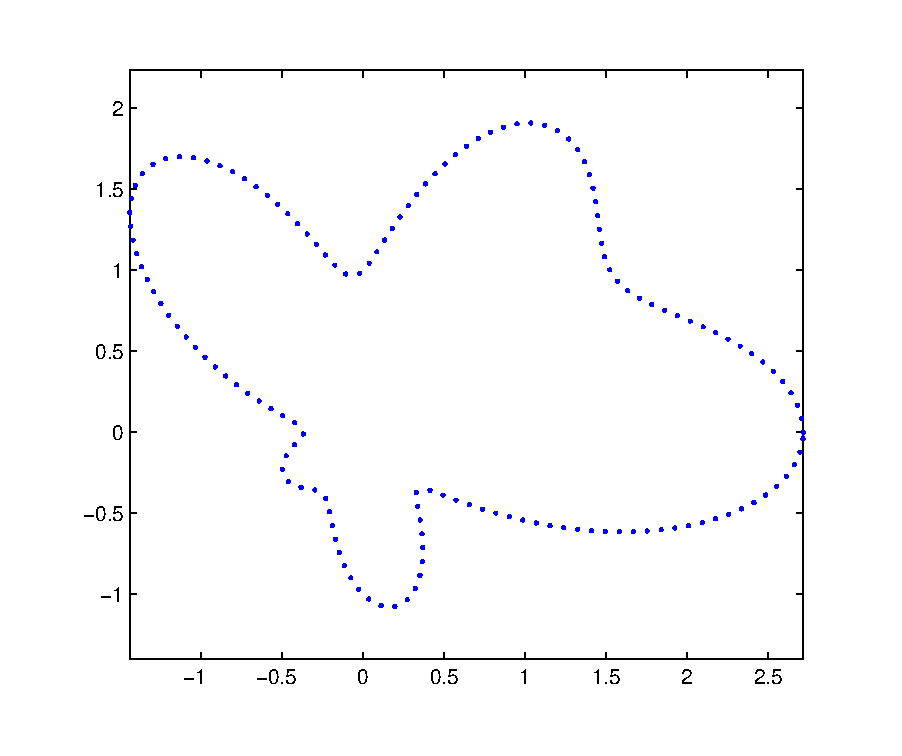
\includegraphics[height=2.5in,width=3.2in]{amoeba_fig.eps}
\end{center}
\caption{The profile of amoeba domain.}\label{fig}%
\end{figure}


\end{document}
